\section{Aggregation}
\label{sect:aggregation}
An inventorisation of aggregates desired by users of validation reports
yielded a wide range of desires\footnote{Inventories were taken at 
the ESSnet Validat Integration meeting in \"Orebro Sweden (14-16 February 2017) and during
the Task Force on Validation meeting in Luxemburg (27 April 2017). Minutes of both
meetings are available via \href{https://ec.europa.eu/eurostat/cros}{CROS-portal} .}.
Commonly reported aggregates include the total number or fraction of rules
violated or the number or fraction of records  that violate a certain rule.
Aggregates need not have a numerical value. For example, in the case of
record-wise validation rules, interesting aggregates include `the validation
rule that is violated most often by a dataset' or the `record violating most
(record-wise) validation rules'. 

Before discussing how we endow machine-readable validation reports with
identifiable and combinable aggregates, it is useful to point out some of the
subtleties that arise when thinking of aggregation in a general way. The first
subtlety has to do with counting rules and counting validation results.
Consider as an example the rules \code{turnover >= 0} and \code{mean(profit) >=
0}.  When applied to a set of $n$ business records containing the variables
\code{turnover} and \code{profit}, the first rule is evaluated $n$ times in $n$
validation events, yielding $n$ validation results. The second rule is
evaluated in a single validation event, yielding a single validation result,
regardless of the number of records in the dataset. This means that an
aggregate such as `the total number of rules violated' is ill-defined. It is
only meaningful to talk about `the number of events that resulted in
\onwaar{}'. 

The second subtlety is that a set of aggregates can again be combined to form
new aggregates. For example, in a first step we may compute the fraction of
events yielding \onwaar{} per economic sector. In a next step we count for how
many sectors this number is less than or equal to 0.05.

Figure~\ref{fig:graphs} illustrates the above points in a graph-like structure.
Suppose we start with a basic report containing five validation results. We can
add an aggregate counting the number of passes in a certain subset
(Figure~\ref{fig:graph1}).  In Figure~\ref{fig:graph2}, a second count is
added, as well as an overall count that is composed of the two low-level
aggregates. Figure~\ref{fig:graph3} depicts a situation where a subset of
validation results is combined to form aggregates of several types: the number
of passes and the fraction of passes.
%
\begin{figure}[!t]
  \centering
  \begin{subfigure}[b]{0.7\textwidth}
    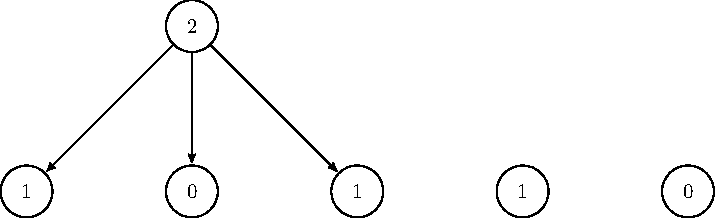
\includegraphics[width=\textwidth]{fig/graph1.pdf}
    \caption{Validation report with a single aggregated value.}
    \label{fig:graph1}
  \end{subfigure}
  \begin{subfigure}[b]{0.7\textwidth}
    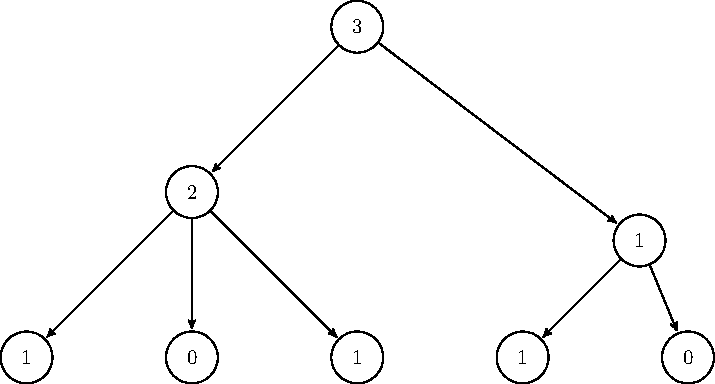
\includegraphics[width=\textwidth]{fig/graph2.pdf}
    \caption{Validation report with multiple aggregates.}
    \label{fig:graph2}
  \end{subfigure}
  \begin{subfigure}[b]{0.7\textwidth}
    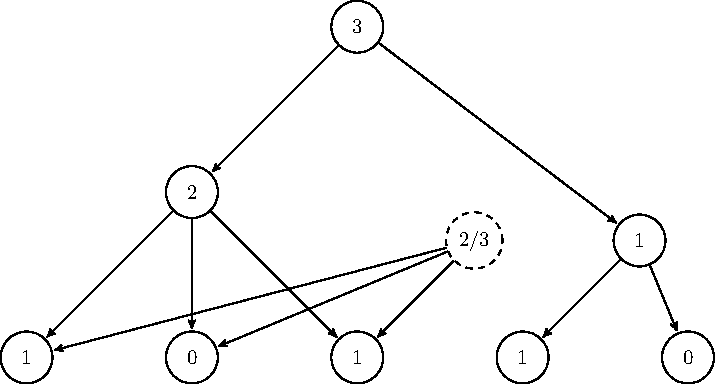
\includegraphics[width=\textwidth]{fig/graph3.pdf}
    \caption{Validation report with aggregates of various types.}
    \label{fig:graph3}
  \end{subfigure}
  \caption{Structure of validation reports including aggregates, of varying complexity.}
  \label{fig:graphs}
\end{figure}

These examples suggest that aggregates can be interpreted as nodes in a
directed graph where the edges (arrows) point from the aggregate to the nodes
used to compute the contents of the node. Nodes that have no outgoing edges
(leaves) correspond one-to-one with validation results.  The collection of
nodes and edges contains sufficient structure to make the representation of
validation reports identifiable, combinable, and (recursively) aggregable. In
the following paragraph we define more closely the type of graph that can be
used to represent an aggregation structure.


%%%%%%%%%%%%%%%%%%%%%%%%%%%%%%%%%%%%%%%%%%%%%%%%%%%%%%%%%%%%%%%%%%%%%%%%%%%%%%%
\subsection{Aggregation graphs}
\label{sect:aggregationgraphs}
Graphs are well-known mathematical structures that represent connectivity
between objects. Indeed, the  study of graphs dates back to the 18th century
when Leonhard \citet{euler1741solutio} solved the famous K\"oningsberger
bridges problem.  For our purposes, a graph will serve as a model to store
validation results, aggregates thereof, and the operations that lead to the
aggregated values.

The need for a graph structure rather then a more simple record-like structure
arises from the demand that reports be combinable to a new report.  To see
this, consider the following example. Two institutes validate a dataset with
turnover values against the rule \code{turnover >= 0}. The first institute
reports the fraction of passes, while the second institute reports the results
for each individual record. If these reports were naively combined, one could
misinterpret the fractional value reported by the first institute as pertaining
to the separate values reported by the second institute. A second example
occurs when the first institute creates a report containing both the individual
results and the aggregated fraction of passes. If this report is to be
augmented with new information, for example when new records come in it should
be clear from the report that the reported fraction of passes does not pertain
to the records added later.


Graphs basically consist of elements of some set, called \emph{nodes} or
\emph{vertices} and connections between them, which are called \emph{edges} or
\emph{arrows} if they are directed. Structured information can be stored by
endowing the nodes and edges with parcels of data.  Depending on the type and
number of edges allowed between the nodes, graphs are classified in a broad
number of types.  Below we define simple directed graph that comes close to our
purpose of structuring validation aggregates.
%
\begin{definition}
\label{def:simplegraph}
A \emph{simple finite directed graph} is a pair  $(V,E)$ where $V$ is a finite set and $E$
is a set of pairs $(v_1,v_2)$ with $v_1,v_2\in V$ and $v_1\not=v_2$.
\end{definition}
The term \emph{directed} means
that edges have a direction: the edge $(v_1,v_2)$ can be thought of as an
arrow, pointing from $v_1$ to $v_2$ and therefore differs from ($v_2$,$v_1$).
The first element of an edge is referred to as the \emph{start} and the second
element is referred to as the \emph{end} of the edge. In a simple
directed graph there are no loops (edges whose start and end are the same)
and there are maximally two opposite-pointing edges that connect two
nodes.

A validation report can be represented by a more special graph. To define it,
we first need the concept of a paths and cycles.
\begin{definition}[path, cycle]
\label{def:pathcycle}
A \emph{path} is a sequence of edges edges $e_1,e_2,\ldots,e_n$ such that the 
end of $e_j$ is equal to the start of
$e_{j+1}$ for $j=1,2,\ldots,n-1$. A \emph{cycle} is a path such that the end of
$e_n$ is equal to the start of $e_1$.
\end{definition}
A path is thus a sequence of connected edges. Since aggregation works bottom-up
and not top-down, we define the following graph to represent an extended
validation report.
\begin{definition}
A \emph{directed acyclic graph} is a simple finite directed graph $(V,E)$ with
the condition that $E$ contains no cycles.
\end{definition}
%
The term `directed acyclic graph' is often shortened to DAG in literature. This
particular structure has many technical applications, For example, the DAG
stands model for data processing flow in the SPARK model for distributed
computing \citep{gupta2003spark}. 


Simple graphs have a natural rule of composition. The `sum' of two simple
(directed) graphs is obtained as the union of the two vertex sets and the union
of the two edge sets. For a DAG, this combination rule does not always apply
since such a combination could in principle introduce cycles. (As an example,
combine the DAGs $({a,b},{(a,b)})$ and $({a,b},{(b,a)})$, the result is no
longer a DAG). We therefore define the following compatibility rule for
directed acyclic graphs.
\begin{definition}[Compatible DAGs]
\label{def:compatibledag}
Given two DAGs $G=(V,E)$ and $F=(V',E')$. These graphs are called
\emph{compatible} when the combination
\begin{align*}
 (V\cup V', E\cup E'),
\end{align*}
is also a DAG.
\end{definition}
A practical consequence of the condition in this definition is that software
that combines extended validation reports (validation reports including
aggregations, to be defined below) should always check for compatibility of the
reports upon combination. 

One case compatible graphs occurs when both $G$ and $F$ are edgeless. Two
reports that do not contain any aggregates satisfy this condition. If and $G$
have no nodes or edges in common, they are also compatible. 


%%%%%%%%%%%%%%%%%%%%%%%%%%%%%%%%%%%%%%%%%%%%%%%%%%%%%%%%%%%%%%%%%%%%%%%%%%%%%%%
\subsection{Identifying aggregates}
Just like validation results, aggregation results are created by evaluating an
expression. Also, just like for validation results, the interpretation of to
what dataset an aggregate pertains need not coincide with the data used to
compute the result. Consider a set of validation results
$\la{v}=(v_1,v_2,\ldots,v_k,v_{k+1},v_{k+2},\ldots, v_n)$. Here,
$v_1\ldots v_k$ pertain to one subset of the data under scrutiny, for example a
certain economic sector, and $v_{k+1},\ldots,v_n$ pertain to another subset.
The aggregate
\begin{align*}
a = k - \sum_{j=1}^{k}v_j,
\end{align*}
counts the number of violations in the first subset. In this case, the
aggregate communicates a fact about the set used in the calculation.
Now consider
\begin{align*}
a' = \frac{a}{n-\sum_{j=1}^n{v_j}}.
\end{align*}
This aggregate is the fraction of all failures that occur in the first subset.
Although every validation result is used to compute it, such aggregates are
usually reported in a table with one column stating the subset (e.g. the
economic sector) and one column stating the aggregate value. 

For this reason it is proposed that the validation report provides explicit
room to communicate cases where by intention, the value set to which an
aggregate pertains are not identical to the values used in evaluation of a
rule. 
%
\begin{definition}[aggregation]
\label{def:aggregation}
An \emph{aggregation} is a tuple  
$(e, d, f, a)$
where $e$ identifies the aggregating event, $d$ the data related to the
aggregation, $f$ the aggregating expression, and $v$ the aggregate value.
\end{definition}
We leave open the possibility that the elements $e$, $d$ and $f$ are again
tuples. In particular, $d$ may identify both the data used while evaluating a
rule and the data to which the aggregate value pertains.  Observe also that the
data element ($d$) fixes the edges of the aggregation graph.  Like
Definition~\ref{def:confrontation}, this is not a definition in a precise
mathematical sense. Rather it is something that can be tested in a particular
practical software/data environment. 


